\documentclass[journal,12pt,twocolumn]{IEEEtran}
\usepackage{amsmath,amssymb,amsfonts,amsthm}
\usepackage{txfonts}
\usepackage{tkz-euclide}
\usepackage{listings}
\usepackage{gvv}
\usepackage[latin1]{inputenc}
\usepackage{array}
\usepackage{pgf}
\usepackage{lmodern}

\begin{document}
\bibliographystyle{IEEEtran}

\vspace{3cm}

\title{}
\author{EE23BTECH11217 - Prajwal M$^{*}$
}
\maketitle
\newpage
\bigskip

\renewcommand{\thefigure}{\theenumi}
\renewcommand{\thetable}{\theenumi}


\section*{Exercise 9.1}

\noindent \textbf{12} \hspace{2pt}Write the five terms at n = 1, 2, 3, 4, 5 of the sequence and obtain the corresponding series

$ x \brak{n} =
\begin{cases}
-1 & n = 1 \\
\frac{x \brak{n-1}}{n} & n \geq 2 \\
 0 & n \leq 0
\end{cases}
$
\\

\noindent Solution:

\noindent
\begin{align*}
x \brak{1} & = -1 \\
x \brak{2} & = \frac{x \brak{1}}{2} = -\frac{1}{2} \\
x \brak{3} & = \frac{x \brak{2}}{3} = -\frac{1}{2   3} = -\frac{1}{6}\\
x \brak{4} & = \frac{x \brak{3}}{4} = -\frac{1}{2   3   4} = -\frac{1}{24}\\
x \brak{5} & = \frac{x \brak{4}}{5} = -\frac{1}{2   3   4   5} = -\frac{1}{120}
\end{align*} \\

% So the first five terms of the series are:
% $$-1 , -\frac{1}{2}, -\frac{1}{6}, -\frac{1}{24},  -\frac{1}{120}$$ \\

The corresponding series:
\begin{align*}
    \sum_{n=-\infty}^{\infty} x \brak{n} & = \ldots + 0 + x \brak{1} + x \brak{2} + x \brak{3} + \ldots \\
    & = \ldots + 0 -1 +   \brak{-\frac{1}{2} } +   \brak{-\frac{1}{6} } + \ldots \\
\end{align*}

The nth term of the series is,
\begin{align*}
    x \brak{n} & = \frac{-1}{n!}  \brak{u \brak{n}}
\end{align*}

\begin{figure}
  \centering
  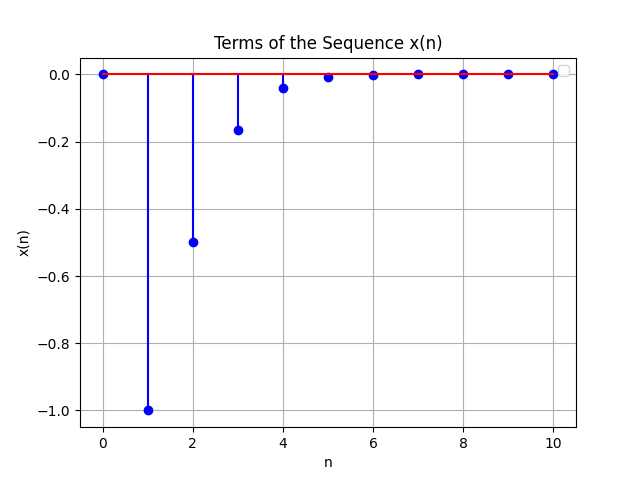
\includegraphics[width=0.5\textwidth]{plot.png}
\end{figure}

The Z-transform of $ x \brak{n} $ is given by:
$$x \brak{n} \ztransform F \brak{z}$$

\begin{align*}
    F \brak{z} & = \sum_{n=-\infty}^{\infty} x \brak{n}   z^{-n} \\
    & = \sum_{n=-\infty}^{\infty} \frac{-1}{n!}  u \brak{n}   z^{-n} \\
    & = \sum_{n=1}^{\infty} \frac{-1}{n!}   z^{-n} \\
    & = -  \brak{e^{z^{-1}} - 1} \\
    & = 1 - e^{z^{-1}}
\end{align*}

So, the Z-transform of the given series is
$ 1 - e^{z^{-1}} $.\\


For the series to converge, the ratio test must be satisfied for n $>$ 0
\begin{align*}
 \lim_{{n \to \infty}}  \left| \frac{x \brak{n+1} z^{- \brak{n+1}}}{x \brak{n} z^{-n}}  \right| & <  1 \\
\lim_{{n \to \infty}}  \left| \frac{-z^{-n-1} n!}{-z^{-n}  \brak{n+1}!} \right| & < 1\\
\lim_{{n \to \infty}}  \left| \frac{z^{-1}}{n+1}  \right| & < 1\\
\end{align*}

The condition is satisfied for $ \text{Re} \brak{z} \neq 0 $ \\

Hence, ROC of Z transform is $$z\in\mathbb{C} : Re \brak{z} \neq 0$$.

\end{document}u
